
\documentclass[xcolor=dvipsnames]{beamer} 
\usetheme{default} 

\usecolortheme[named=Blue]{structure}
\usetheme[height=7mm]{Rochester} 
\setbeamertemplate{items}[ball] 
\setbeamertemplate{blocks}[rounded]
\setbeamertemplate{navigation symbols}{} 

\usepackage{tikz} 
\usetikzlibrary{shapes.arrows,chains,positioning,decorations.pathreplacing,shapes.misc}

% -------------------------------------------------------------------------
% Commands
% -------------------------------------------------------------------------

\newcommand{\addone}[2]{ 
  
  \node (plus1) [inner sep=0pt,draw,circle, fill=blue!50,below= 1em of #1] {\tiny +1};
  \draw (#1) -- (plus1);
  \draw [->] (plus1) -- (#2);   
} 

\newcommand{\sumupPrim}[2]{

  \node (sumup) [inner sep=0pt,draw,circle, fill=blue!50,below= 1em of #1] {\tiny +};
  \draw (#1) -- (sumup);
  \draw [->] (sumup) -- (#2);   
}

\newcommand{\sumup}[2]{

  \node (sumup) [inner sep=0pt,draw,circle, fill=blue!50,below= 1em of #1] {\tiny +};
  \draw (#1) -- (sumup);
  \draw [->] (sumup) |- (#2);   
}

\newcommand{\adder}[3]{ 
  \node (adder) [inner sep=0pt,draw,circle, fill=blue!50,below right= 0.5em and -0.2em of #1] {\tiny +};
  \draw (#1.south) |- (adder); 
  \draw (#2.south) |- (adder); 
  \draw [->] (adder) -- (#3.north);     
} 


\begin{document}

% -------------------------------------------------------------------------
%
% -------------------------------------------------------------------------

\title{Embedded Languages for Data-Parallel Programming} 
\author[J. Svensson]{Bo Joel Svensson} 
\institute{ 
  Department of Computer Science and Engineering \\ 
  Chalmers University of Technology 
} 

% -------------------------------------------------------------------------
%
% -------------------------------------------------------------------------

\begin{frame}[plain] 
  \titlepage
\end{frame} 


\section{background} 

\begin{frame}{Data-Parallelism} 
  \begin{center}
  {\Large Data-Parallelism}
  \end{center}
\end{frame} 


% -------------------------------------------------------------------------
% What is data parallelism ?
%   * Fine grained
%   * Scalable (more data -> more potential for parallelism) 
%   
% -------------------------------------------------------------------------
\begin{frame}{Data-Parallelism: Increment}
\begin{center} 
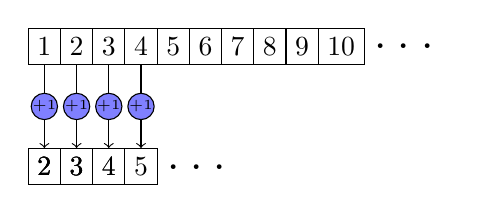
\begin{tikzpicture}[
      start chain=1 going right,start chain=2 going below,node distance=-0.15mm
    ]


  \foreach \x in {1,2,...,10} {
    \node (\x) [draw, on chain=1] {\x};
  }
  \node [on chain=1] {\huge \ldots};
  
  

  \onslide<2>{
    \node [draw, below=3em of 1] (r1) {2};
    % \draw [->] (1) -- (r1);
    \addone{1}{r1}
    }

  \onslide<3>{
    \node [draw, below=3em of 1] (r1) {2};
    \node [draw, below=3em of 2] (r2) {3};
    %\draw [->] (2) -- (r2);
    \addone{2}{r2}
    }


  \onslide<4>{
    \node [draw, below=3em of 1] (r1) {2};
    \node [draw, below=3em of 2] (r2) {3};
    \node [draw, below=3em of 3] (r3) {4};
    %\draw [->] (3) -- (r3);
    \addone{3}{r3}
    }

  \onslide<5>{
    \node [draw, below=3em of 1] (r1) {2};
    \node [draw, below=3em of 2] (r2) {3};
    \node [draw, below=3em of 3] (r3) {4};
    \node [draw, below=3em of 4] (r4) {5};
    %\draw [->] (4) -- (r4);
    \addone{4}{r4}
    \node [right=-0.15mm of r4] {\huge \ldots};
    }
  
\end{tikzpicture} 
\end{center}
\end{frame}

% -------------------------------------------------------------------------
%
% -------------------------------------------------------------------------
\begin{frame}{Data-Parallelism: Increment in Parallel}
\begin{center} 
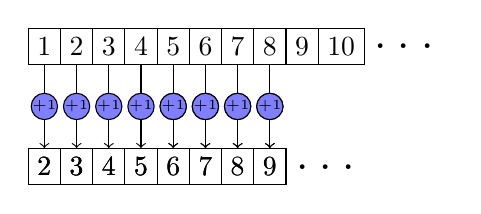
\begin{tikzpicture}[
      start chain=1 going right,start chain=2 going below,node distance=-0.15mm
    ]


  \foreach \x in {1,2,...,10} {
    \node (\x) [draw, on chain=1] {\x};
  }
  \node [on chain=1] {\huge \ldots};
  
  

  \onslide<2>{
    \node [draw, below=3em of 1] (r1) {2};
    \node [draw, below=3em of 2] (r2) {3};
    \node [draw, below=3em of 3] (r3) {4};
    \node [draw, below=3em of 4] (r4) {5};

    \addone{1}{r1}
    \addone{2}{r2}
    \addone{3}{r3}
    \addone{4}{r4}
    }

  \onslide<3>{
    \node [draw, below=3em of 1] (r1) {2};
    \node [draw, below=3em of 2] (r2) {3};
    \node [draw, below=3em of 3] (r3) {4};
    \node [draw, below=3em of 4] (r4) {5};
    \node [draw, below=3em of 5] (r5) {6};
    \node [draw, below=3em of 6] (r6) {7};
    \node [draw, below=3em of 7] (r7) {8};
    \node [draw, below=3em of 8] (r8) {9};

    \addone{5}{r5}
    \addone{6}{r6}
    \addone{7}{r7}
    \addone{8}{r8}
    }

  \onslide<3>{
    \node [draw, below=3em of 1] (r1) {2};
    \node [draw, below=3em of 2] (r2) {3};
    \node [draw, below=3em of 3] (r3) {4};
    \node [draw, below=3em of 4] (r4) {5};
    \node [draw, below=3em of 5] (r5) {6};
    \node [draw, below=3em of 6] (r6) {7};
    \node [draw, below=3em of 7] (r7) {8};
    \node [draw, below=3em of 8] (r8) {9};

    \addone{5}{r5}
    \addone{6}{r6}
    \addone{7}{r7}
    \addone{8}{r8}

    \node [right=-0.15mm of r8] {\huge \ldots};
    }

\end{tikzpicture} 

\end{center}
\end{frame}

% -------------------------------------------------------------------------
% Computing a sum
% -------------------------------------------------------------------------
\begin{frame}{Data-Parallelism: Sum}
\begin{center} 
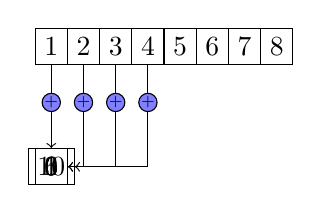
\begin{tikzpicture}[
      start chain=1 going right,start chain=2 going below, node distance=-0.15mm
    ]


  \foreach \x in {1,2,...,8} {
    \node (\x) [draw, on chain=1] {\x};
  }
  
  
  \onslide<2>{
    \node [draw, below=3em of 1] (r1) {0};
  
    }

  
  \onslide<3>{
    \node [draw, below=3em of 1] (r1) {1};
  
    \sumupPrim{1.south}{r1.north}
    }
  
  \onslide<4>{
    \node [draw, below=3em of 1] (r1) {3};
  
    \sumup{2.south}{r1.east}
    }
  
  \onslide<5>{
    \node [draw, below=3em of 1] (r1) {6};
  
    \sumup{3.south}{r1.east}
    }

  \onslide<6>{
    \node [draw, below=3em of 1] (r1) {10};
    \sumup{4.south}{r1.east}
    }




\end{tikzpicture} 
\end{center}
\end{frame}

% -------------------------------------------------------------------------
% Computing a sum in parallel 
% -------------------------------------------------------------------------

\begin{frame}{Data-Parallelism: Sum in Parallel}
\begin{center} 
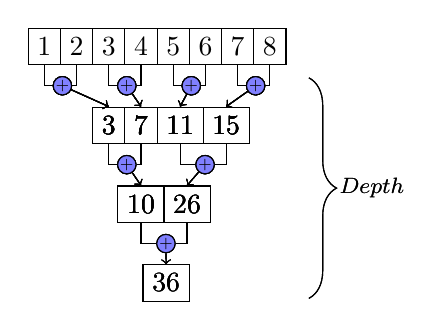
\begin{tikzpicture}[
      start chain=1 going right,start chain=2 going below,node distance=-0.15mm
    ]


  \foreach \x in {1,2,...,8} {
    \node (\x) [draw, on chain=1] {\x};
  }
  
  \onslide<2>{
    \node (imm1) [draw,below=1.5em of 3] {3};
    \node (imm2) [draw,right= of imm1] {7};
    \node (imm3) [draw,right= of imm2] {11};
    \node (imm4) [draw,right= of imm3] {15};
    
    \adder{1}{2}{imm1}
    \adder{3}{4}{imm2}
    \adder{5}{6}{imm3}
    \adder{7}{8}{imm4}
   
  }

  \onslide<3>{
    \node (imm1) [draw,below=1.5em of 3] {3};
    \node (imm2) [draw,right= of imm1] {7};
    \node (imm3) [draw,right= of imm2] {11};
    \node (imm4) [draw,right= of imm3] {15};

    \adder{1}{2}{imm1}
    \adder{3}{4}{imm2}
    \adder{5}{6}{imm3}
    \adder{7}{8}{imm4}
   
    \node (jmm1) [draw,below=1.5em of imm2] {10};
    \node (jmm2) [draw,right= of jmm1] {26};

    \adder{imm1}{imm2}{jmm1}
    \adder{imm3}{imm4}{jmm2} 
  }

 \onslide<4>{
    \node (imm1) [draw,below=1.5em of 3] {3};
    \node (imm2) [draw,right= of imm1] {7};
    \node (imm3) [draw,right= of imm2] {11};
    \node (imm4) [draw,right= of imm3] {15};

    \adder{1}{2}{imm1}
    \adder{3}{4}{imm2}
    \adder{5}{6}{imm3}
    \adder{7}{8}{imm4}

    \node (jmm1) [draw,below=1.5em of imm2] {10};
    \node (jmm2) [draw,right= of jmm1] {26};

    \adder{imm1}{imm2}{jmm1}
    \adder{imm3}{imm4}{jmm2}

    \node (lmm1) [draw,below right=1.5em and -0.8em of jmm1] {36};
    
    \adder{jmm1}{jmm2}{lmm1} 
  }

  \onslide<5>{
    \node (imm1) [draw,below=1.5em of 3] {3};
    \node (imm2) [draw,right= of imm1] {7};
    \node (imm3) [draw,right= of imm2] {11};
    \node (imm4) [draw,right= of imm3] {15};

    \adder{1}{2}{imm1}
    \adder{3}{4}{imm2}
    \adder{5}{6}{imm3}
    \adder{7}{8}{imm4}

    \node (jmm1) [draw,below=1.5em of imm2] {10};
    \node (jmm2) [draw,right= of jmm1] {26};

    \adder{imm1}{imm2}{jmm1}
    \adder{imm3}{imm4}{jmm2}

    \node (lmm1) [draw,below right=1.5em and -0.8em of jmm1] {36};
    
    \adder{jmm1}{jmm2}{lmm1}

    \draw [decorate,
           decoration={brace,mirror,amplitude=10pt},xshift=-4pt,yshift=0pt]
          (3.5,-3.2) -- (3.5,-0.4) node [black,midway,xshift=0.8cm]  
          {\footnotesize $Depth$};
  }

 \onslide<6>{
    \node (imm1) [draw,below=1.5em of 3] {3};
    \node (imm2) [draw,right= of imm1] {7};
    \node (imm3) [draw,right= of imm2] {11};
    \node (imm4) [draw,right= of imm3] {15};

    \adder{1}{2}{imm1}
    \adder{3}{4}{imm2}
    \adder{5}{6}{imm3}
    \adder{7}{8}{imm4}

    \node (jmm1) [draw,below=1.5em of imm2] {10};
    \node (jmm2) [draw,right= of jmm1] {26};

    \adder{imm1}{imm2}{jmm1}
    \adder{imm3}{imm4}{jmm2}

    \node (lmm1) [draw,below right=1.5em and -0.8em of jmm1] {36};
    
    \adder{jmm1}{jmm2}{lmm1}

    \draw [decorate,
           decoration={brace,mirror,amplitude=10pt},xshift=-4pt,yshift=0pt]
          (3.5,-3.2) -- (3.5,-0.4) node [black,midway,xshift=0.8cm]  
          {\footnotesize $Depth$};
         
  }
\end{tikzpicture} 

\onslide<6>{
   \begin{tikzpicture}[overlay,remember picture] 
      
    \node [fill=red!50,single arrow] at (-3.7,3.5) {\tiny Potential for parallelism};
    \node [fill=red!50,single arrow] at (-2.8,2.4) {\tiny Potential for parallelism};
    \end{tikzpicture}
 
}


\end{center}
\end{frame}

% -------------------------------------------------------------------------
%
% -------------------------------------------------------------------------

\begin{frame}{Data-Parallelism}

  \begin{columns} 

  \begin{column}{.48\textwidth}
  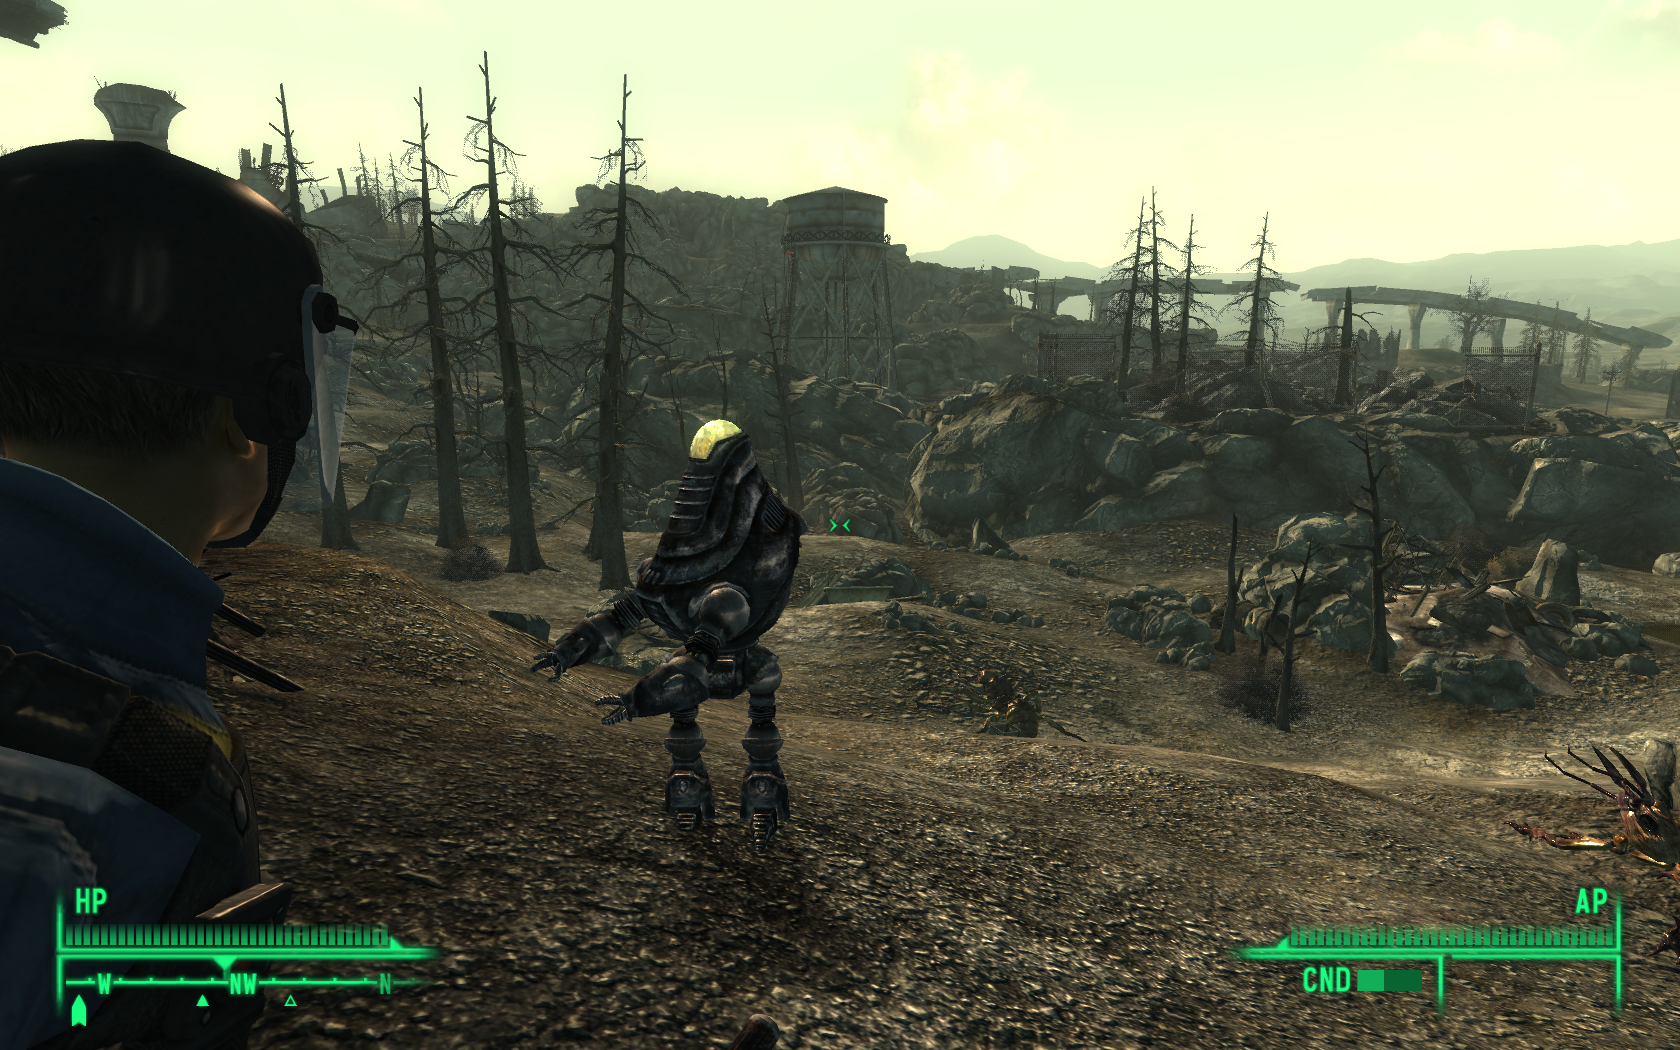
\includegraphics[width=\linewidth]{fallout.jpg}

  Rendering

  \vspace{1cm}
  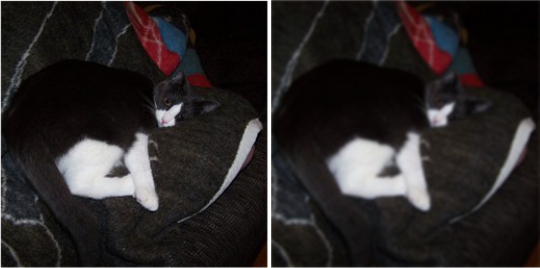
\includegraphics[width=\linewidth]{kiri.jpg}

  Image processing

  \end{column} 
  
  \begin{column}{.48\textwidth} 
  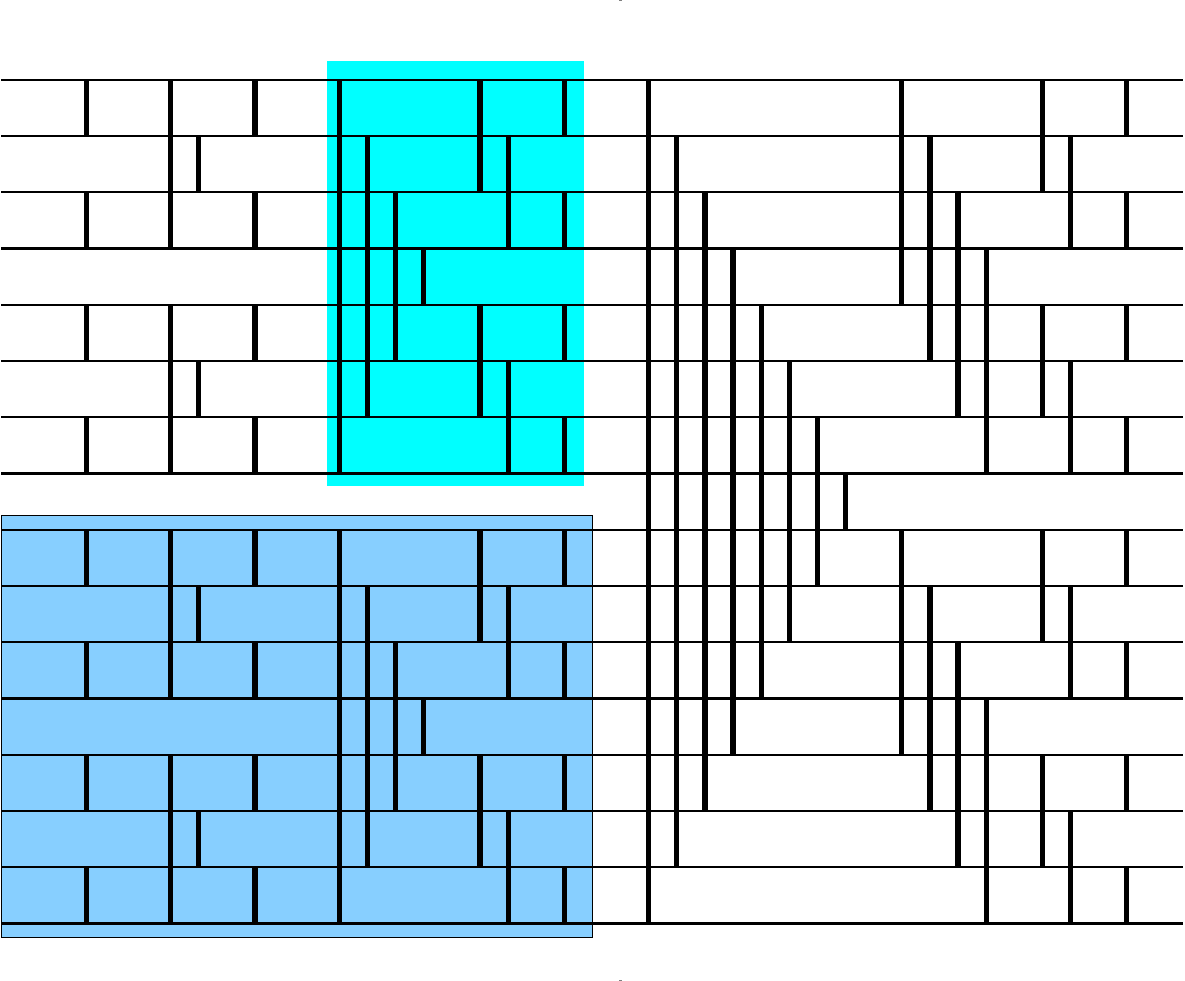
\includegraphics[width=\linewidth]{mmixedsorter.pdf}

  Sorting

  \end{column}
  
  \end{columns}

\end{frame}


\begin{frame}{Data-Parallelism}

  \begin{itemize} 
    \item Scalable
      \begin{itemize} 
        \item Potential for parallelism increases with data size 
      \end{itemize}
    \item Fine grained parallelism 
  \end{itemize} 

\end{frame}

% -------------------------------------------------------------------------
%
% -------------------------------------------------------------------------
\section{GPUs and CUDA}

\begin{frame}{GPUs} 

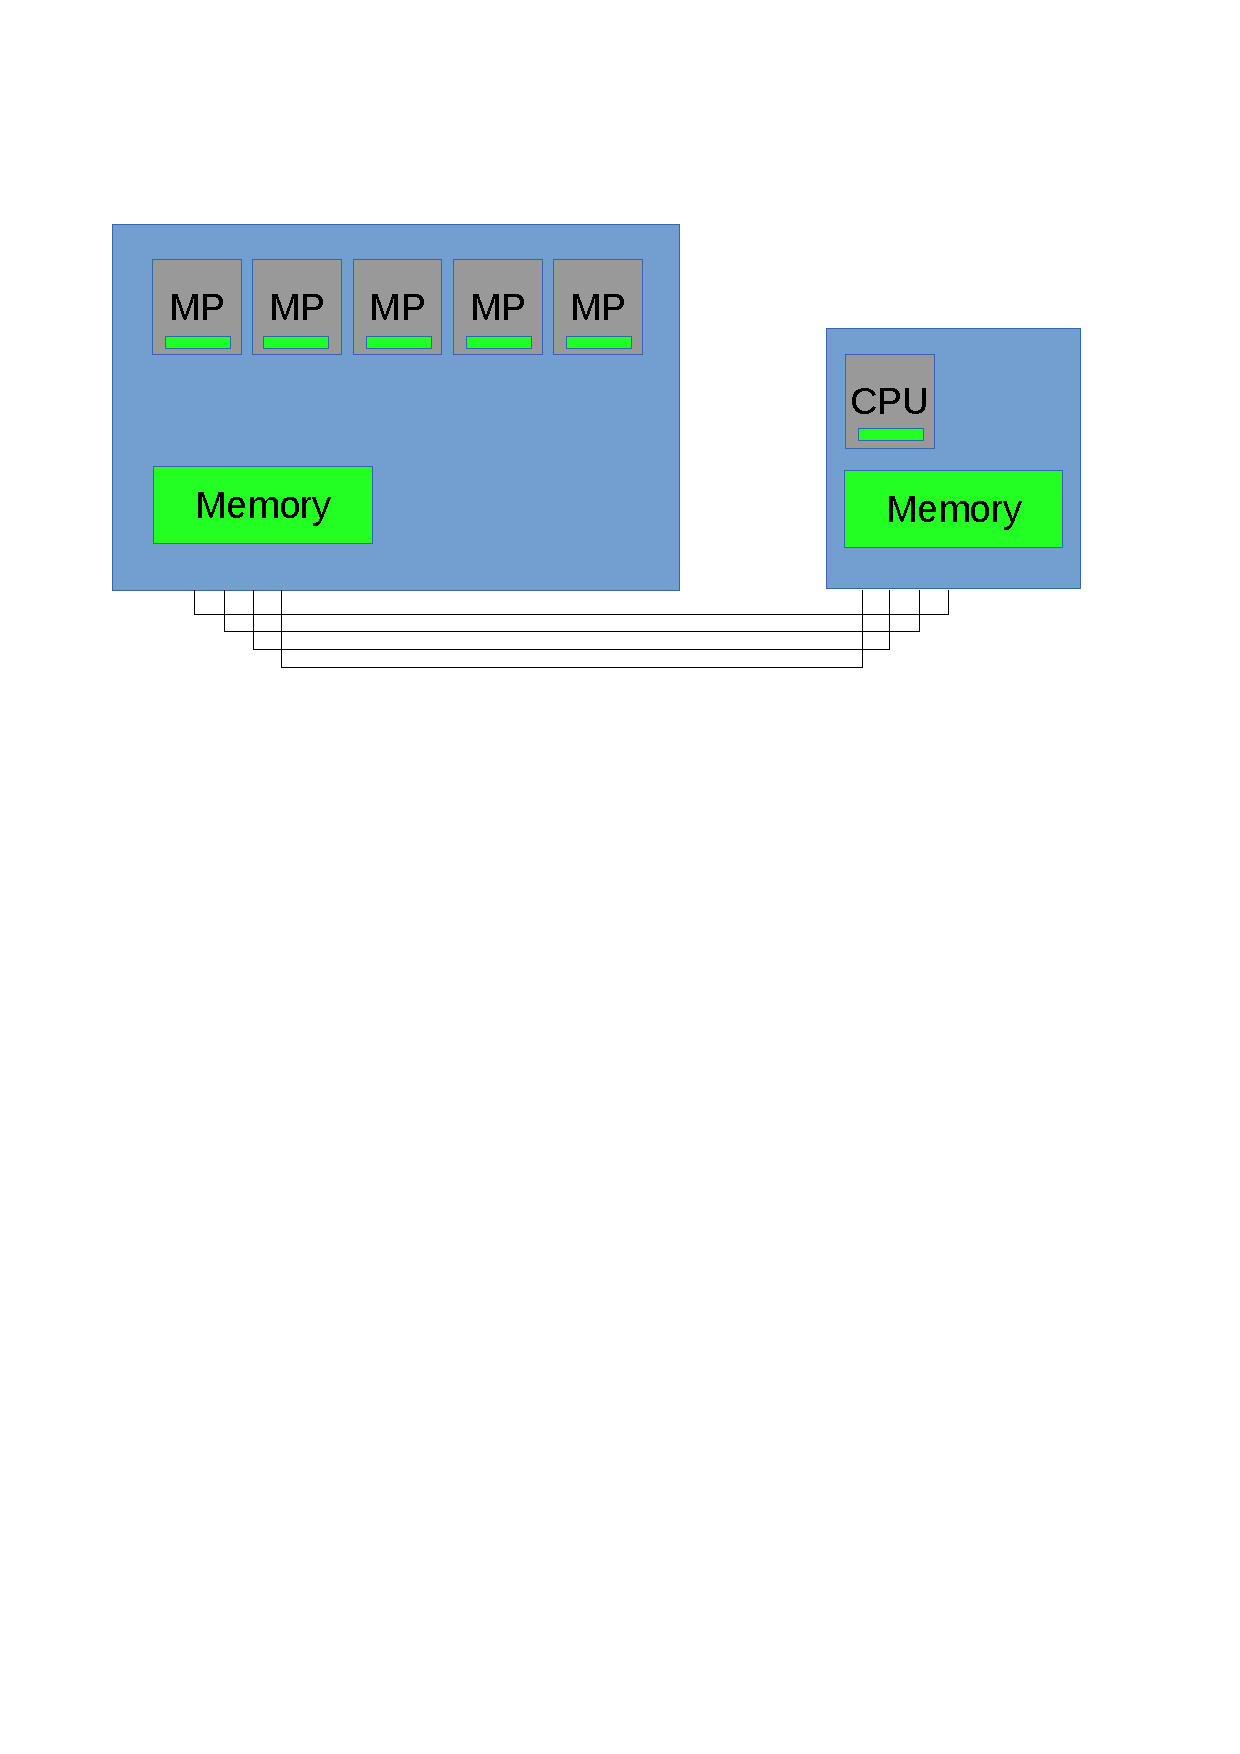
\includegraphics[width=\linewidth]{GPU1.pdf}


\end{frame} 

\begin{frame}{GPUs} 

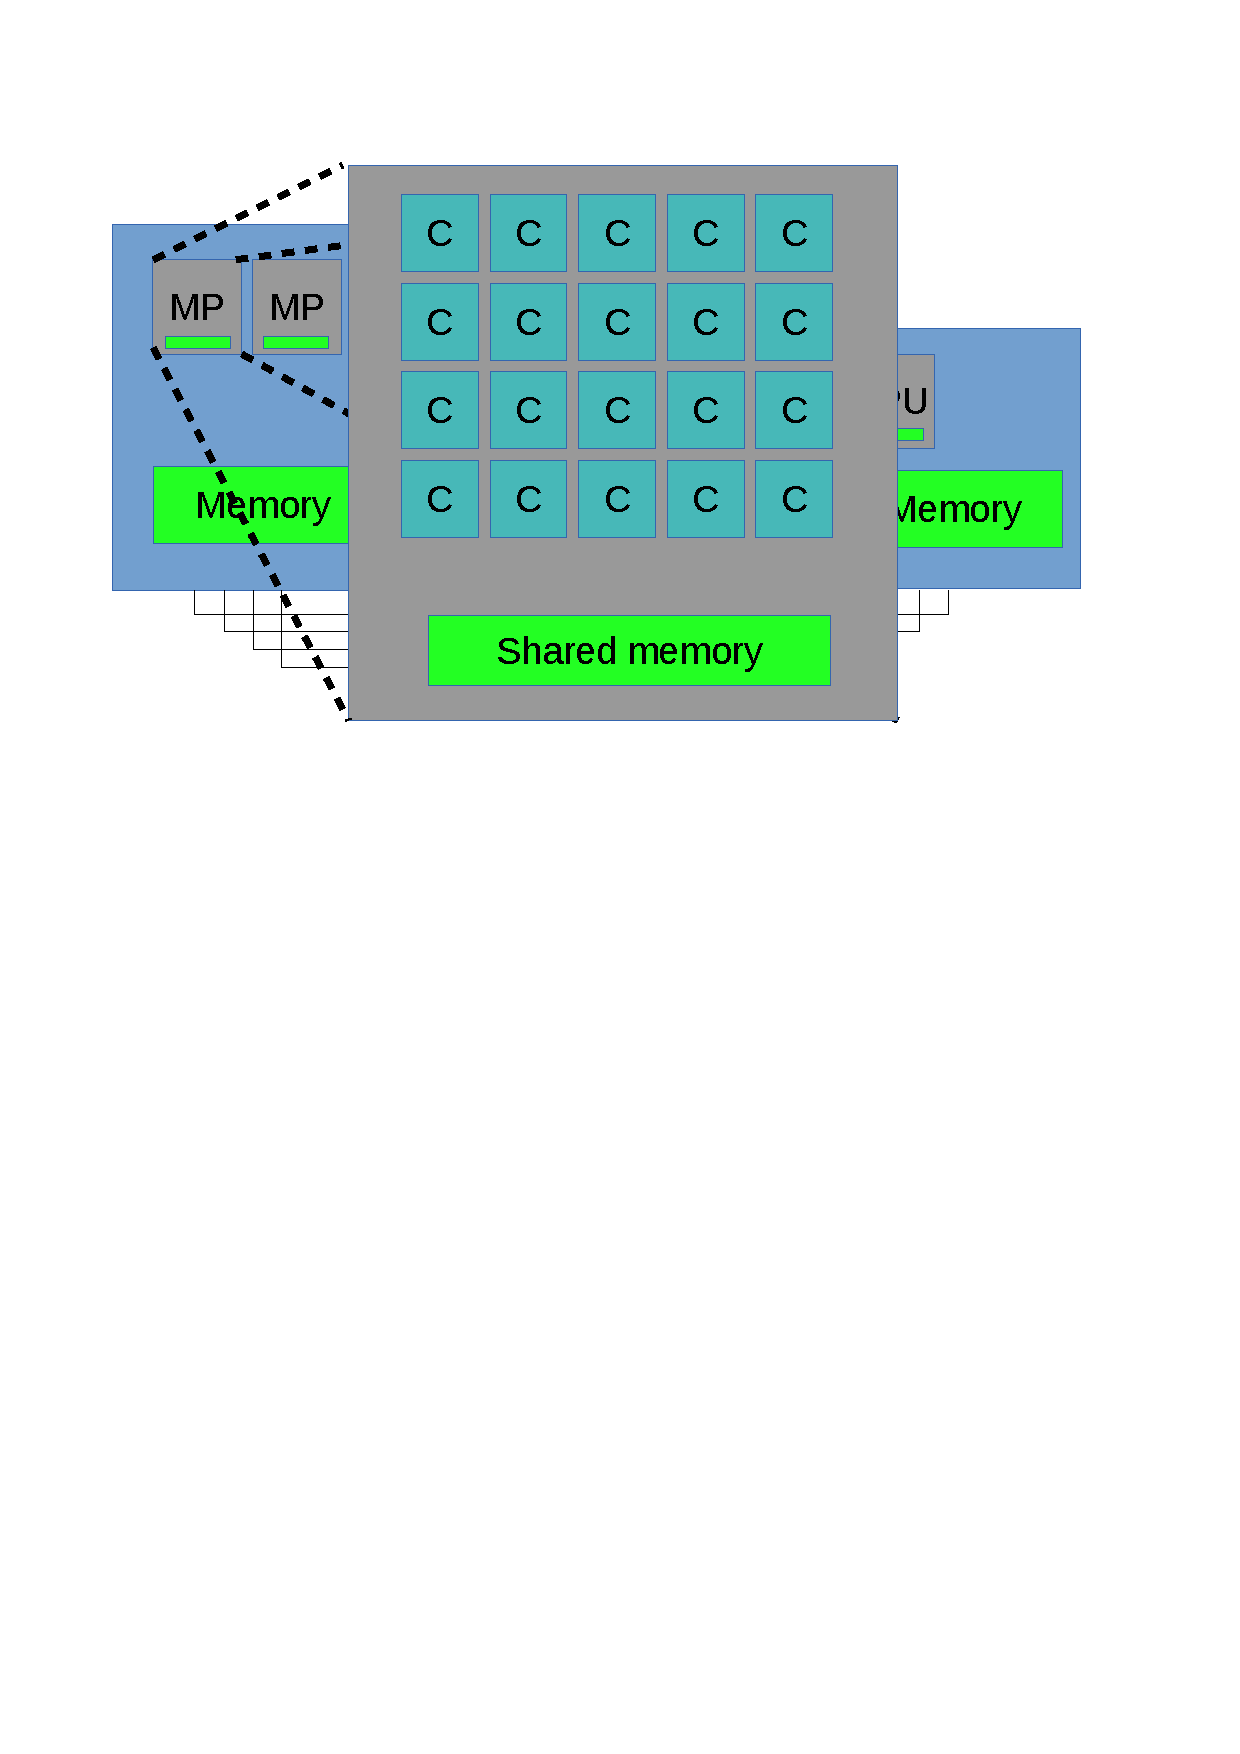
\includegraphics[width=\linewidth]{GPU2.pdf}


\end{frame} 


% -------------------------------------------------------------------------
%
% -------------------------------------------------------------------------


\begin{frame}{GPU Programming}
\begin{center} 

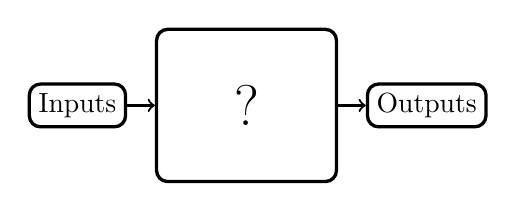
\begin{tikzpicture}[
      start chain=1 going right,start chain=2 going below,node distance=1em,
      every join/.style={->,thick},
    ]

  \node [draw,very thick, rounded corners, on chain=1,join] {Inputs}; 
  \node [draw,very thick, rounded corners, on chain=1,minimum height=5.5em,minimum width = 6.5em,join] {\huge ?}; 
  \node [draw,very thick, rounded corners, on chain=1,join] {Outputs}; 
  

\end{tikzpicture} 
\end{center}

\end{frame}

% -------------------------------------------------------------------------
%
% -------------------------------------------------------------------------

\begin{frame}{GPU Programming}
\begin{center} 

\begin{tikzpicture}[remember picture,
      start chain=going right,
      outer/.style={on chain, node distance=1em},
      every join/.style={->,thick},
      inner/.style={circle,draw=blue!50,fill=blue!20,thick,inner sep=1pt},
    ]

  \node [outer,draw,very thick, rounded corners,join] {Inputs}; 
  \node [outer,draw=gray!50,very thick, rounded corners,minimum height=5.5em,minimum width = 6.5em,join] (apa) {
    \begin{tikzpicture} 
      \node [draw=black!100,inner,minimum size=1pt] (k1) {k1};
      \node [draw=black!100,inner,minimum size=1pt, below= 1em of k1] (k2) {k2};
      \node [draw=black!100,inner,minimum size=1pt, right= 1em of k1] (k3) {k3}; 
    \end{tikzpicture}

  }; 
  \node [outer,draw,very thick, rounded corners,join] {Outputs}; 
  

  \draw (k1) -- (k3)
        (k2) -- (k3)
        (apa.west) -- (k1.west)
        (apa.west) -- (k2.west) 
        (k3.east) -- (apa.east); 
  

\end{tikzpicture} 

\onslide<2-3>{
  \begin{tikzpicture}[overlay, remember picture]
    
   \node [draw, circle,very thick, minimum size=2em] (magni) at (-0.58,2.05) {};
    
   \node [draw, very thick] (test) at (-1,0) {
     \begin{tikzpicture}
       \node [draw, fill=red!50] (b0) {Block 0};
       \node [draw, fill=red!50, below=0pt of b0] (b1) {Block 1};
       \node [below=0pt of b1] (bdots) {\huge \ldots};
       \node [draw, fill=red!50, below=0pt of bdots] (bN) {Block N};
       

     \end{tikzpicture} 

   };

   \draw [very thick] (magni) -- (test);
  \end{tikzpicture}
}

\onslide<3>{ 
  
\begin{tikzpicture}[overlay, remember picture]
    \node [fill=gray!50] at (2,0) {
      \begin{minipage}{3.5cm}
      Block:
      \begin{small}
      \begin{itemize}
        \item Many threads
        \item Shared memory
        \item Synchronize
        \item Same program 
        \item Different data
      \end{itemize}
      \end{small}
      \end{minipage}
    };
  \end{tikzpicture}
}



\end{center}

\end{frame}

% -------------------------------------------------------------------------
%
% -------------------------------------------------------------------------
\begin{frame}[fragile]{GPU Programming: CUDA Example}

\begin{block}{}
\begin{verbatim} 
__global__ void inc(int32_t *a, int32_t *r) {
  
  unsigned int gid = blockIdx.x * 
                     blockDim.x + 
                     threadIdx.x;

  r[gid] = a[gid] + 1; 

} 
\end{verbatim}
\end{block} 


\end{frame} 

% -------------------------------------------------------------------------
%
% -------------------------------------------------------------------------
\begin{frame}[fragile]{GPU Programming: CUDA Example}

\begin{block}{}
\begin{tiny}
\begin{verbatim} 
main(void) {
  
  int32_t h_a[32], h_r[32]; 
  int32_t *d_a, *d_r;
  
  for (int i = 0; i < 32; ++i) 
    h_a[i] = i;

  cudaMalloc((void**)&d_a,32*sizeof(int32_t));
  cudaMalloc((void**)&d_r,32*sizeof(int32_t));

  cudaMemcpy(d_a,h_a,32*sizeof(int32_t),
                     cudaMemcpyHostToDevice);
  
  inc<<<1,32,0>>>(d_a,d_r); 

  cudaMemcpy(h_r,d_r,32*sizeof(int32_t),
                     cudaMemcpyDeviceToHost);

  for (int i = 0; i < 32; ++i) 
    printf("%d ",h_r[i]);
}
\end{verbatim}
\end{tiny}
\end{block} 
\end{frame} 
% -------------------------------------------------------------------------
%
% -------------------------------------------------------------------------

\begin{frame}{GPU Programming} 

  Things to consider:

  \begin{itemize} 
    \item Minimise data transfer between host and device
    \item Coalesce global memory accesses
    \item Minimise use of global memory 
    \item Avoid different execution paths within a block
    \item Be careful with {\tt \_\_syncthreads} and conditionals
  \end{itemize} 
  
\end{frame} 


% -------------------------------------------------------------------------
%
% -------------------------------------------------------------------------
\section{Embedded Languages: Background}


\begin{frame}{Embedded Languages} 
 \begin{center}
   {\Large Compiled Embedded Languages}
 \end{center}
%%
%%  Embedding ArBB, similar slides to Obsidian, more pictures. 

\end{frame} 


\begin{frame}[fragile]{Embedded Languages: Background} 
  
  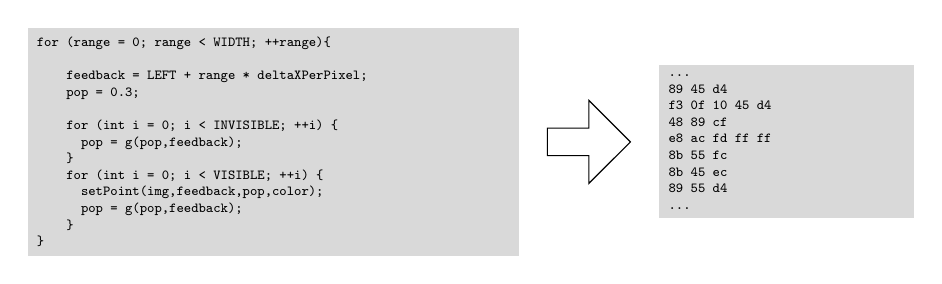
\begin{tikzpicture} 

    \node [fill=gray!30] (cuda) {
      \begin{minipage}{6cm}
        \begin{tiny} 
\begin{verbatim}
for (range = 0; range < WIDTH; ++range){

    feedback = LEFT + range * deltaXPerPixel;
    pop = 0.3;

    for (int i = 0; i < INVISIBLE; ++i) {
      pop = g(pop,feedback);
    }
    for (int i = 0; i < VISIBLE; ++i) {
      setPoint(img,feedback,pop,color);
      pop = g(pop,feedback);
    }
}
\end{verbatim}    
\end{tiny}    
\end{minipage}
};
    \node [draw,single arrow,right=1em of cuda, minimum size=3em] (arr) {};
    
    \node [fill=gray!30,right=1em of arr] (mc) { 
      \begin{minipage}{3cm}
\begin{tiny}
\begin{verbatim}
...
89 45 d4             
f3 0f 10 45 d4
48 89 cf
e8 ac fd ff ff
8b 55 fc      
8b 45 ec      
89 55 d4      
...
\end{verbatim}
\end{tiny}
      \end{minipage}
    };
      
      
    
  \end{tikzpicture}

  
\end{frame} 

% -------------------------------------------------------------------------
%
% -------------------------------------------------------------------------
\begin{frame}{Embedded Languages} 

  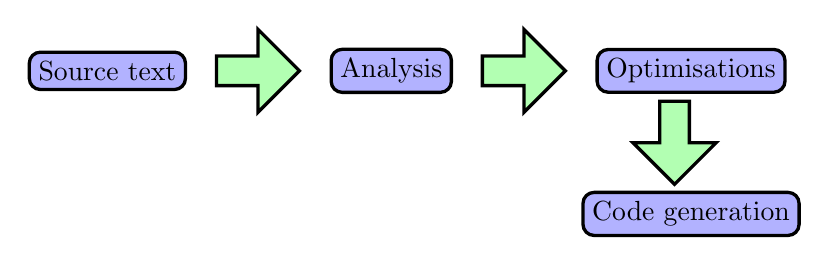
\begin{tikzpicture} 
    
    %\onslide<1-5>{
    \node [draw, fill=blue!30, very thick, rounded corners] 
      (source) {Source text}; 
    %}
    \onslide<2-5>{ 
      \node [draw, fill=green!30, 
             very thick, 
             minimum size = 3em,
             single arrow, 
             right=1em of source] (a1) {};

      \node [draw, fill=blue!30, 
             very thick, rounded corners, 
             right=1em of a1] (analysis) {Analysis};
    }
    \onslide<4-5>{
      
      \node [draw, fill=green!30, 
             very thick, 
             minimum size = 3em,
             single arrow, 
             right=1em of analysis] (a1) {};
      
      \node [draw, fill=blue!30, 
             very thick, rounded corners, 
             right=1em of a1] (opt) {Optimisations};
      
    }
    \onslide<5>{
       \node [draw, fill=green!30, 
             very thick, 
             minimum size = 3em,
             single arrow, rotate=270, 
             below=1.5em of opt] (a1) {};
      
      \node [draw, fill=blue!30, 
             very thick, rounded corners, 
             below=3.5em of opt] (codegen) {Code generation}; 
    }

  \end{tikzpicture}

  \onslide<3>{ 
    \begin{tikzpicture}[overlay, remember picture] 
      \node [draw] at (5,0) (details1) {
         \begin{tikzpicture} 
           \node (text1) {``2 * a + 1''}; 
           \node [draw, thick, 
                  single arrow, 
                  minimum size=2em, right=1em of text1] 
           (localarr) {};
           \node [draw, circle,thick,inner sep=1pt] (pnode) at (4,0.7) {$+$};
           \node [draw, circle,thick,inner sep=2pt, below left=1em and 1em of pnode](mnode)  {$*$}; 
           \draw (pnode) -- (mnode);

           \node [below left=1em and 1em of mnode] (two) {$2$};
           \node [below right=1em and 1em of mnode] (anode) {$a$}; 
           \node [below right=1em and 1em of pnode] (onenode) {$1$};

           \draw (mnode) -- (two) 
                 (mnode) -- (anode) 
                 (pnode) -- (onenode); 
           
         \end{tikzpicture} 
        };
    \end{tikzpicture}
  }

%       + 
%   *       1 
% 2   a 

\end{frame} 

% -------------------------------------------------------------------------
%
% -------------------------------------------------------------------------
\begin{frame}{Embedded Languages} 

  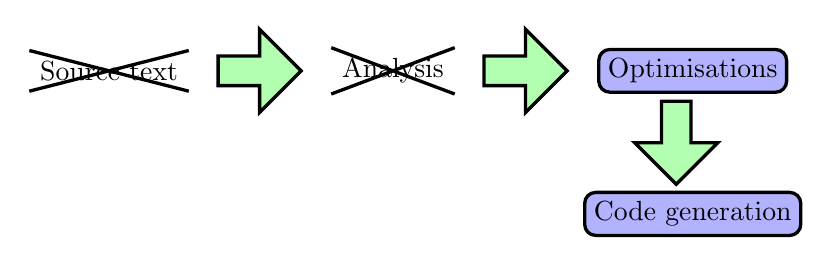
\begin{tikzpicture} 
    
    \node [draw, very thick, cross out] 
      (source) {Source text}; 
    
    \node [draw, fill=green!30, 
           very thick, 
           minimum size = 3em,
           single arrow, 
           right=1em of source] (a1) {};

    \node [draw, cross out, 
           very thick,
           right=1em of a1] (analysis) {Analysis};

    
    \node [draw, fill=green!30, 
           very thick, 
           minimum size = 3em,
           single arrow, 
           right=1em of analysis] (a1) {};
      
    \node [draw, fill=blue!30, 
           very thick, rounded corners,
           right=1em of a1] (opt) {Optimisations};
      
    \node [draw, fill=green!30, 
           very thick, 
           minimum size = 3em,
           single arrow, rotate=270, 
           below=1.5em of opt] (a1) {};
      
    \node [draw, fill=blue!30, 
           very thick, rounded corners, 
           below=3.5em of opt] (codegen) {Code generation}; 
    
  \end{tikzpicture}

  \begin{tikzpicture}[overlay, remember picture]     
    \node [draw, fill=blue!30, 
           very thick, rounded corners] at (8.55,4.75) (lib) {Library};
    \node [draw, fill=green!30, 
           very thick, 
           minimum size = 3em,
           single arrow, rotate=270, 
           below right=0.8em and -1em of lib] (a1) {};
    
  \end{tikzpicture} 

\end{frame} 


% -------------------------------------------------------------------------
%
% -------------------------------------------------------------------------
\begin{frame}[fragile]{Embedded Languages: {\small Embedded Four-Function Calculator}}

\begin{block}{}
\begin{verbatim} 
import Prelude hiding (div) 
import qualified Prelude as P

data Op = Add | Sub | Mul | Div 

data Expr = Bin Expr Op Expr | Lit Int 

eval (Bin e1 op e2) =
  let (e1', e2') = (eval e1, eval e2) in
    case op of Add -> e1' + e2'
               Sub -> e1' - e2'
               Mul -> e1' * e2'
               Div -> e1' `P.div` e2'

eval (Lit i) = i
\end{verbatim}  
\end{block} 

\end{frame} 

% -------------------------------------------------------------------------
%
% -------------------------------------------------------------------------
\begin{frame}[fragile]{Embedded Languages: {\small Embedded Four-Function Calculator}} 

\begin{block}{}
\begin{verbatim} 
instance Num Expr where
  (+) a b = Bin a Add b 
  (-) a b = Bin a Sub b
  (*) a b = Bin a Mul b 
  fromInteger = Lit . fromInteger

div a b = Bin a Div b 
\end{verbatim}  
\end{block} 

\end{frame} 

% -------------------------------------------------------------------------
%
% -------------------------------------------------------------------------
\begin{frame}[fragile]{Embedded Languages: {\small Embedded Four-Function Calculator}} 

\begin{block}{}
\begin{verbatim} 
ex1 :: Expr
ex1 = 9*1+2
\end{verbatim}  
\end{block} 

\pause
\begin{block}{}
\begin{verbatim} 
ex2 :: Expr -> Expr
ex2 x = a + a 
  where
    a = x*x
\end{verbatim}  
\end{block} 

\pause
\begin{block}{}
\begin{verbatim} 
ex3 :: Expr
ex3 = P.sum (map fromInteger [0..15])
\end{verbatim}  
\end{block} 

\end{frame} 


% -------------------------------------------------------------------------
%
% -------------------------------------------------------------------------
\section{Obsidian}

% -------------------------------------------------------------------------
%
% -------------------------------------------------------------------------



\begin{frame}{Obsidian} 
  
  \begin{center}
  {\Large Embedded Language for GPU Kernel Implementation}
  \end{center}
  %% \begin{itemize} 
  %%   \item Our level of GPU programming 
  %%   \item Programming example  (reduction) 
  %%   \item Performance 
  %%   \item Compare to related approaches 
  %% \end{itemize}
      
\end{frame} 

% -------------------------------------------------------------------------
%
% -------------------------------------------------------------------------

\begin{frame}{Obsidian} 
  Obsidian: 
  \begin{itemize} 
    \item Encourage experimentation
    \item Higher level than CUDA 
      \begin{itemize} 
        \item Not as much indexing magic
        \item Programs describe ``whole'' computation
        \item Code reuse 
        \item Still have control over low level details
      \end{itemize} 
  \end{itemize}  
\end{frame}

% -------------------------------------------------------------------------
%
% -------------------------------------------------------------------------

\begin{frame}[fragile]{Obsidian: Simple Example}

\begin{block}{} 
\begin{verbatim} 
inc :: Num a => SPull a -> SPull a
inc = fmap (+1)
\end{verbatim} 
\end{block} 

\pause 
\begin{block}{} 
\begin{verbatim} 
incK :: Num a => DPull (SPull a) -> DPush Grid a
incK arr = pConcatMap (push . inc) arr
\end{verbatim} 
\end{block} 


\end{frame} 

% -------------------------------------------------------------------------
%
% -------------------------------------------------------------------------
\newcommand\Fontvi{\fontsize{8}{7.2}\selectfont}

\begin{frame}[fragile]{Obsidian: Generated Code}
\begin{block}{256 threads and 256 elements per block} 
\Fontvi
\begin{verbatim} 
extern "C" __global__ void inc(int32_t* input0, uint32_t n0,
                               int32_t* output1)
{
    uint32_t tid = threadIdx.x;
     
    if (blockIdx.x < n0 / 256U) {
        output1[blockIdx.x * 256U + tid] = 
          input0[blockIdx.x * 256U + tid] + 1;
    }
}
\end{verbatim} 

\end{block}
\end{frame}

% -------------------------------------------------------------------------
%
% -------------------------------------------------------------------------
\begin{frame}[fragile]{Obsidian: Generated Code}
\begin{block}{128 threads and 256 elements per block}
\Fontvi
\begin{verbatim} 
extern "C" __global__ void inc(int32_t* input0, uint32_t n0,
                               int32_t* output1)
{
    uint32_t tid = threadIdx.x;
    
    if (blockIdx.x < n0 / 256U) {
        for (int i = 0; i < 2; ++i) {
            tid = i * 128 + threadIdx.x;
            output1[blockIdx.x * 256U + tid] = 
              input0[blockIdx.x * 256U + tid] + 1;
        }
        tid = threadIdx.x;
    }
}
\end{verbatim} 
\end{block} 


\end{frame} 

\begin{frame}[fragile]{Obsidian: Execute Generated Code}
  
  \begin{block}{}
    \Fontvi
\begin{verbatim}
perform =
  withCUDA $
  do
    kern <- capture 256 (incK . splitUp 256) 

    useVector (V.fromList [0..255 :: Int32]) $ \i ->
      useVector (V.fromList (P.replicate 256 (0 :: Int32))) $ \ o ->
      do
        o <== (1,kern) <> i 
        r <- peekCUDAVector o
        lift $ putStrLn $ show r     
\end{verbatim} 
  \end{block}
\end{frame} 
% -------------------------------------------------------------------------
%
% -------------------------------------------------------------------------
\begin{frame}{Related Work: Accelerate} 
\begin{center} 

\begin{tikzpicture}[remember picture,
      start chain=going right,
      outer/.style={on chain, node distance=1em},
      every join/.style={->,thick},
      inner/.style={circle,draw=blue!50,fill=blue!20,thick,inner sep=1pt},
    ]

  \node [outer,draw,very thick, rounded corners,join] {Inputs}; 
  \node [outer,draw=gray!50,very thick, rounded corners,minimum height=5.5em,minimum width = 6.5em,join] (apa) {
    \begin{tikzpicture} 
      \node [draw=black!100,inner,minimum size=1pt] (k1) {k1};
      \node [draw=black!100,inner,minimum size=1pt, below= 1em of k1] (k2) {k2};
      \node [draw=black!100,inner,minimum size=1pt, right= 1em of k1] (k3) {k3}; 
    \end{tikzpicture}

  }; 
  \node [outer,draw,very thick, rounded corners,join] {Outputs}; 
  

  \draw (k1) -- (k3)
        (k2) -- (k3)
        (apa.west) -- (k1.west)
        (apa.west) -- (k2.west) 
        (k3.east) -- (apa.east); 
  

\end{tikzpicture} 

\onslide<2>{ 
  \begin{tikzpicture}[overlay, remember picture]
    \node [draw,fill=gray!50,thick, rounded corners] at (-3,-1) {
      \begin{minipage}{5cm} 
        Accelerate: 
         \begin{itemize}  
         \item ks are chosen from a set of primitives
           \begin{itemize}
             \item Map
             \item Fold
             \item Permute
             \item .. 
           \end {itemize} 
         \item Coordination / Composition
         \end{itemize}
      \end{minipage} 
      
    };
  \end{tikzpicture} 
} 
\end{center}
\end{frame} 

% ---------------------------------------------------------------------------
%
% ---------------------------------------------------------------------------

\begin{frame}{Related Work: Accelerate}
\begin{center} 

\begin{tikzpicture}[remember picture,
      start chain=going right,
      outer/.style={on chain, node distance=1em},
      every join/.style={->,thick},
      inner/.style={circle,draw=blue!50,fill=blue!20,thick,inner sep=1pt},
    ]

  \node [outer,draw,very thick, rounded corners,join] {Inputs}; 
  \node [outer,draw=gray!50,very thick, rounded corners,minimum height=5.5em,minimum width = 6.5em,join] (apa) {
    \begin{tikzpicture} 
      \node [draw=black!100,inner,minimum size=1pt] (k1) {k1};
      \node [draw=black!100,inner,minimum size=1pt, below= 1em of k1] (k2) {k2};
      \node [draw=black!100,inner,minimum size=1pt, right= 1em of k1] (k3) {k3}; 
    \end{tikzpicture}

  }; 
  \node [outer,draw,very thick, rounded corners,join] {Outputs}; 
  

  \draw (k1) -- (k3)
        (k2) -- (k3)
        (apa.west) -- (k1.west)
        (apa.west) -- (k2.west) 
        (k3.east) -- (apa.east); 
  

\end{tikzpicture} 

  \begin{tikzpicture}[overlay, remember picture]
    
   \node [draw, circle,very thick, minimum size=2em] (magni) at (-0.58,2.05) {};
    
   \node [draw, very thick] (test) at (-1,0) {
     \begin{tikzpicture}
       \node [draw, fill=red!50] (b0) {Block 0};
       \node [draw, fill=red!50, below=0pt of b0] (b1) {Block 1};
       \node [below=0pt of b1] (bdots) {\huge \ldots};
       \node [draw, fill=red!50, below=0pt of bdots] (bN) {Block N};
       

     \end{tikzpicture} 

   };

   \draw [very thick] (magni) -- (test);
  \end{tikzpicture}

  \begin{tikzpicture}[overlay, remember picture]
    \node [draw,fill=gray!50,thick, rounded corners] at (3,-1) {
      \begin{minipage}{5cm} 
        Obsidian: 
         \begin{itemize}  
         \item Program what the ks do
         \end{itemize}
      \end{minipage} 
      
    };
  \end{tikzpicture} 



\end{center}
\end{frame} 

% ---------------------------------------------------------------------------
%
% ---------------------------------------------------------------------------

\begin{frame}{}
  Reduction example \\
  Performance
\end{frame} 
    



% -------------------------------------------------------------------------
%
% -------------------------------------------------------------------------
\section{EmbArBB} 

\begin{frame}{EmbArBB} 
 \begin{center}
   {\Large Embedding Array Building Blocks in Haskell}
 \end{center}
%%
%%  Embedding ArBB, similar slides to Obsidian, more pictures. 

\end{frame} 

% -------------------------------------------------------------------------
%
% -------------------------------------------------------------------------

\begin{frame}{EmbArBB: ArBB} 

  Intel Array Building Blocks
  \begin{itemize}
    \item Heterogeneous multi/many core systems
    \item High-level programming model 
    \item JIT compile for current architecture   
  \end{itemize}
\end{frame} 


% -------------------------------------------------------------------------
%
% -------------------------------------------------------------------------
\begin{frame}{EmbArBB: ArBB} 
  
  \begin{center} 
  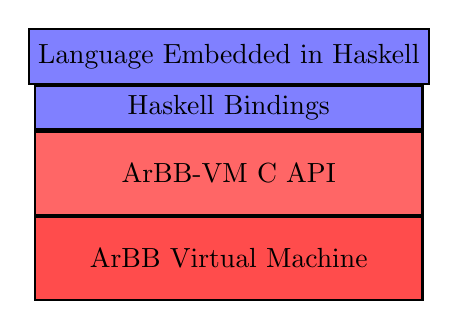
\begin{tikzpicture} 
    
    \node [draw,thick, fill=red!70, minimum width = 14em, 
           minimum height = 3em] 
       (vm)  {ArBB Virtual Machine}; 

    \onslide<2-5>{

    \node [draw,thick, fill=red!60, minimum width = 14em, 
           minimum height = 3em, above= 0pt of vm] 
       (capi) {ArBB-VM C API}; 
    }

    \onslide<3>{

    \node [draw,thick, fill=red!50, minimum width = 14em, 
           minimum height = 3em, above= 0pt of capi] 
       (cpp) {Language Embedded in C++}; 
    }
    
    \onslide<4-5> { 
      \node [draw,thick, fill=blue!50, minimum width = 14em, 
        minimum height = 1em, above= 0pt of capi] 
        (bindings) {Haskell Bindings}; 
    }
    \onslide<5> { 
      \node [draw,thick, fill=blue!50, minimum width = 14em, 
        minimum height = 2em, above= 0pt of bindings] 
        (embarbb) {Language Embedded in Haskell}; 
    }

    
    
  \end{tikzpicture}
  \end{center} 

\end{frame} 

% -------------------------------------------------------------------------
%
% -------------------------------------------------------------------------

\begin{frame}{} 
  Programming example 
\end{frame} 

\begin{frame}{} 

  Performance
\end{frame} 



% -------------------------------------------------------------------------
%
% -------------------------------------------------------------------------
\section{Future Work}
\begin{frame}{Future work} 

\end{frame} 

\begin{frame}{}
  End
\end{frame} 


\end{document} 
